\chapter{Entwicklungsstartegie}
\label{chap:git-strat}

Das Projekt wird auf mehreren Branches entwickelt um eine saubere Trennung zwischen Entwickung und produktivem Code zu gewährleisten. Dazu wird auf die GitFlow branching Strategie gesetzt. Hierbei gibt es zwei Hauptbranches: 

Zum einen den main branch der den produktiven Code enthält und dessen build Artifakte in die prokutive Umgebung deployed werden und den develop Branch auf dem die aktive Entwicklung stattfindet. Einzellne features werden auf so gennanten Feature-Branches entwickelt. Ist ein Feature fertig entwickelt, kann es auf dem develop branch integriert werden. Auf dem develop branch können dann auch umfassendere Tests laufen die sicher stellen, dass das zurück merges des Feature-Branches nicht zu einer Destabilisierung des gesammt Systems geführt hat. Wenn der develop Branch alle Tests duchlaufen hat und alle Features die für den nächsten Release gewünscht waren fertig entwickelt sind, wird der develop in den main Branch zurück gemerged, was zu einem neuen Release führt.

Zusätzlich gibt es für schnelle Paches von wichtigen Fehlern die Möglichkeit hotfix Branches anzulegen, die direkt in den main Branch gemerged werden dürfen.

Wenn mehrere Entwickler an einem Projektm das eine solche Branching-Strategie verfolgt, arbeiten, dann sollten Branch-Protection-Rules eingesetzt werden um die beiden Hauptbranches zu schützen. So bietet es sich z.B. an dann für einen Merge auf develop oder main immer ein Reviewer einen den Pull-Request genehmigen muss. Außderdem kann es sinnvoll sein, dass bestimmte Tests nicht ausfallen dürfen bevor auf den develop oder main branch gemerged wird.

\begin{figure}
    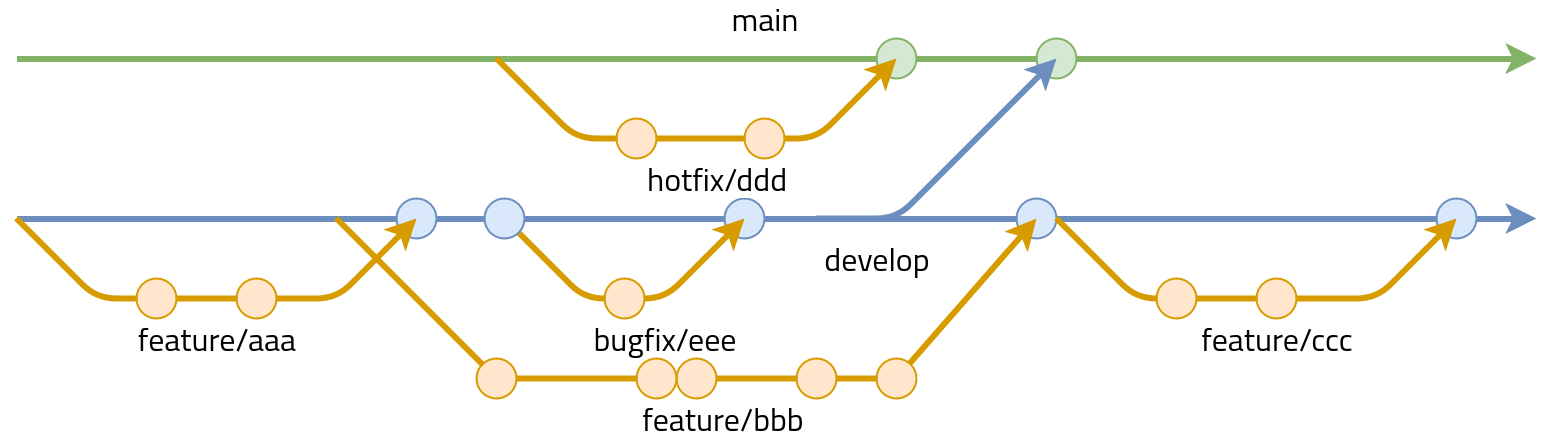
\includegraphics[scale=0.25]{res/branching_scheme.drawio.png}
    \caption{Vereinfachte Darstellung eines Branch-Graphs bei Anwendung des beschriebenen Branching Schemas.}
\end{figure}